\documentclass[conference]{IEEEtran}
\IEEEoverridecommandlockouts
% The preceding line is only needed to identify funding in the first footnote. If that is unneeded, please comment it out.
\usepackage[utf8]{inputenc}
\usepackage[vietnamese]{babel}
\usepackage{float}
\usepackage{cite}
\usepackage{amsmath,amssymb,amsfonts}
\usepackage{algorithmic}
\usepackage{graphicx}
\usepackage{textcomp}
\usepackage{xcolor}
\usepackage{array}
\usepackage[table]{xcolor}
\usepackage{multirow}
\usepackage{multicol}
\usepackage{mathabx} 

\def\BibTeX{{\rm B\kern-.05em{\sc i\kern-.025em b}\kern-.08em
    T\kern-.1667em\lower.7ex\hbox{E}\kern-.125emX}}
\begin{document} 

\title{DỰ BÁO GIÁ KHOÁNG SẢN SỬ DỤNG CÁC KỸ THUẬT PHÂN TÍCH CHUỖI THỜI GIAN \\
{\footnotesize \textsuperscript{*}Note: Sub-titles are not captured in Xplore and should not be used}
\thanks{Identify applicable funding agency here. If none, delete this.}
} 

\author{
\IEEEauthorblockN{1\textsuperscript{st} Trần Kim Thanh\IEEEauthorrefmark{1},
2\textsuperscript{nd} Mai Quốc Bảo\IEEEauthorrefmark{1},
3\textsuperscript{rd} Bùi Hữu Bằng\IEEEauthorrefmark{1},\\
4\textsuperscript{th} Trần Minh Hoàng\IEEEauthorrefmark{1},
5\textsuperscript{th} and Võ Ngọc Lệ Xuân\IEEEauthorrefmark{1} 
}
\IEEEauthorblockA{\IEEEauthorrefmark{1}Khoa Hệ thống thông tin, Trường đại học Công nghệ thông tin, Đại học Quốc gia Thành phố Hồ Chí Minh, Vietnam \\
Email: 21522605@gm.uit.edu.vn, 21521850@gm.uit.edu.vn, 21520151@gm.uit.edu.vn, 21522101@gm.uit.edu.vn, 21521692@gm.uit.edu.vn} 

}





\begin{abstract}
Trong nhiều thập kỷ gần đây, kim loại quý đã và đang duy trì được sức hút của mình trong giới đầu tư, đặc biệt là vàng, bạch kim và bạc. Cùng với đó, những bài toán và mô hình dự đoán giá kim loại không ngừng được sinh ra và cải tiến với độ chính xác ngày một cao hơn. Tuy vậy, tùy theo bối cảnh kinh tế thế giới và sự tiến bộ của các kỹ thuật phân tích dữ liệu mà những mô hình dự đoán sẽ cho ra những kết quả khác nhau. Để giải quyết vấn đề này, nhóm chúng em sẽ thực hiện xây dựng và đánh giá song song các mô hình dự báo giá theo chuỗi thời gian với 10 thuật toán sau: Linear Regression, ARIMA, RNN, GRU, LSTM, FFT, TBATS, SES, N-HiTS, PatchTST; cùng với đó là 3 phương pháp kiểm định mô hình: MAPE, RMSE, MAE.
\end{abstract} 

\begin{IEEEkeywords}
Linear Regression – Hồi quy tuyến tính, ARIMA – Autoregressive Integrated Moving Average, RNN – Recurrent Neural Network, GRU – Gated Recurrent Unit, LSTM – Long Short Term Memory, FFT – Fast Fourier Transform, TBATS – (Trigonometric seasonality, Box-Cox transformation, ARMA errors, Trend, Seasonal components), SES – Simple Exponential Smoothing, N-HiTS – Neural Hierarchical Interpolation for Time Series, PatchTST – Patch Time Series Transformer, MAPE – Mean Absolute Percentage Error, RMSE – Root Mean Squared Error, MAE – Mean Absolute Error.
\end{IEEEkeywords} 

\section{Giới thiệu chung}
Sự biến động của giá vàng(Au), bạc(Ag) và bạch kim(Pt) luôn là điểm nóng trong lĩnh vực đầu tư và tài chính. Việc dự đoán giá của các loại kim loại quý này không chỉ có ý nghĩa quan trọng trong việc hỗ trợ quyết định đầu tư của các nhà đầu tư và phân tích thị trường, mà còn trong việc cung cấp thông tin chi tiết và chính xác về biến động giá, giúp cải thiện đáng kể hiệu suất kinh doanh và quản lý rủi ro trong các lĩnh vực liên quan như chứng khoán và tiền tệ. \\ 
Dự đoán giá kim loại quý như vàng không chỉ tập trung vào dự đoán giá toàn cầu  của 1 ngày hôm sau mà còn dự đoán giá trong tương lai xa hơn như 3 đến 5 tháng sau, dự đoán khoảng biến động giá, xu hướng biến động, mối liên hệ của giá các kim loại,... Do đó, nhiều trang điện tử dự báo chuyên nghiệp đã được thiết lập như Bloomberg, Kitco, LBmMA,... \\
              Bằng cách so sánh và kiểm định nhiều phương pháp và mô hình dự báo từ kinh điển cho đến mới nhất, nhóm nghiên cứu kỳ vọng sẽ tìm ra được mô hình, thuật toán với kết quả khả quan nhất nhằm linh hoạt đáp ứng được nhu cầu ngày một cao của thị trường. Bài nghiên cứu của chúng em sử dụng bộ dữ liệu từ trang thông tin điện tử MetalPriceAPI để lấy giá vàng, bạch kim, bạc được ghi nhận trong quá khứ (lấy theo mệnh giá USD). 
\section{Các nghiên cứu gần đây} 

\subsection{Nghiên cứu của nhóm tác giả Tawum Juvert Mbah, Haiwang Ye, Jianhua Zhang & Mei Long} 

Nghiên cứu này đã chọn ra sáu yếu tố ảnh hưởng đến thị trường đá vôi để mô phỏng và dự đoán xu hướng giá trong tương lai, bao gồm xi măng, vàng, than đá, năng lượng, lãi suất và giá đá vôi. Nghiên cứu sử dụng hai mô hình mạng nơ-ron sâu tiên tiến là RNN và ARIMA để mô phỏng và dự đoán giá đá vôi. Kết quả cho thấy, mô hình ARIMA đã có dự đoán tốt hơn so với mô hình RNN về xu hướng và biến động giá của đá vôi. Sự khác biệt chính giữa hai mô hình này nằm ở việc mô hình ARIMA có khả năng tạo ra kết quả chính xác hơn và thời gian huấn luyện ít hơn so với mô hình RNN. Do đó, mạng ARIMA được chứng minh là một phương pháp tinh vi và hiệu quả trong việc mô hình, phân tích và dự đoán giá của thị trường đá vôi. 

\subsection{Nghiên cứu của Bojun Yin, Renguang Zuo, Yihui Xiong}
Các nhà nghiên cứu sử dụng mô hình GRU để tạo bản đồ tiềm năng khoáng sản (Mineral Prospectivity Mapping - MPM) , sử dụng dữ liệu từ quận Baguio, Philipines. Các kết quả thu được nhấn mạnh tính hiệu quả của mô hình GRU trong MPM. Các khu vực cao điểm được phân biệt thể hiện mối quan hệ không gian chặt chẽ với các mỏ khoáng sản đã biết, cung cấp thông tin quan trọng cho các hoạt động khai thác khoáng sản tiếp theo trong khu vực nghiên cứu. 
\subsection{Nghiên cứu của F.Javier Galán-Sales, Pablo Reina-Jiménez, Manuel Carranza-García, José María Luna-Romera}
Nghiên cứu tiềm năng của việc sử dụng FFT như một công cụ biến đổi đặc trưng để cải thiện độ chính xác và hiệu quả của các mô hình dự báo chuỗi thời gian. Kết quả của nhóm nghiên cứu cho thấy rằng việc sử dụng FFT như một công cụ biến đổi đặc trưng vượt trội hơn các phương pháp biến đổi đặc trưng truyền thống trong việc dự báo độ chính xác và hiệu quả tính toán.
\section{Tài nguyên} 

\subsection{Các tập dữ liệu sử dụng }\label{AA}
Bộ ba dataset thể hiện giá ba loại kim loại quý: vàng, bạc và platium trong khoảng thời gian từ 1/1/2018 đến 1/3/2024 được lấy nguồn từ các API do \url{https://metalpriceapi.com/} cung cấp. 

Sau khi gọi API để lấy dữ liệu, nhóm tiến hành chuyển đổi từ dạng json thành csv và thu được 3 file csv gồm: 
\begin{itemize}
    \item Giá vàng: \texttt{gold\_price\_2018\_2024.csv}
    \item Giá bạc: \texttt{silver\_price\_2018\_2024.csv}
    \item Giá platinum: \texttt{platium\_price\_2018\_2024.csv}
\end{itemize}
Trong mỗi tập dữ liệu gồm hai cột: 
\begin{itemize}
    \item \textbf{Date}: ngày thu nhập dữ liệu (định dạng YYYY-MM-DD).  
    \item \textbf{Value (USD per troy ounce)}: giá của kim loại quý tương ứng với cột Date (mệnh giá USD).
\end{itemize} 

\subsection{Thống kê miêu tả }
\begin{table}[H]
  \centering
  \caption{Thống kê mô tả giá vàng, giá bạc và giá platinum}
\begin{tabular}{|>{\columncolor{red!20}}c|c|c|c|}
    \hline
     \rowcolor{red!20} & Giá vàng & Giá bạc & Giá platinum \\ \hline
     Count & 2252 & 2251 & 2252 \\ \hline
     Mean & 1673.567 & 20.531 & 940.485\\ \hline
     Std & 262.337 & 4.131 & 106.855\\ \hline
     Min & 1178.57 & 12.112 & 591.46\\ \hline
     25\% & 1419.73 & 16.572 & 864.475\\ \hline
     50\% & 1768.317 & 21.584 & 930.843\\ \hline
     75\% & 1884.517 & 23.975 & 999.513\\ \hline
     Max & 2085.54 & 29.748 & 1306.684\\ \hline
\end{tabular}
\end{table}


\begin{figure}[H]
    \centering
    \begin{minipage}{0.23\textwidth}
    \centering
    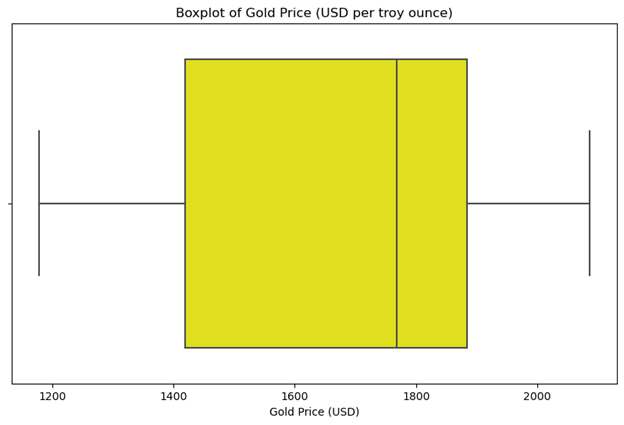
\includegraphics[width=1\textwidth]{bibliography/Figure/boxplot_gold.png}
    \caption{Biểu đồ hộp của giá vàng}
    \label{fig:1}
    \end{minipage}
    \hfill
    \begin{minipage}{0.23\textwidth}
    \centering
    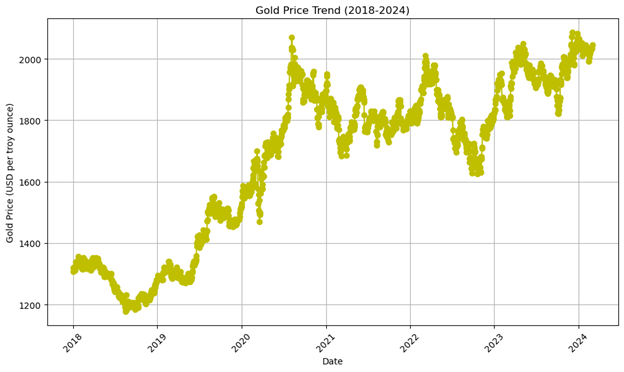
\includegraphics[width=1\textwidth]{bibliography/Figure/line_gold.png}
    \caption{Biểu đồ đường của giá vàng}
    \label{fig:2}
    \end{minipage}
\end{figure} 

\begin{figure}[H]
    \centering
    \begin{minipage}{0.23\textwidth}
    \centering
    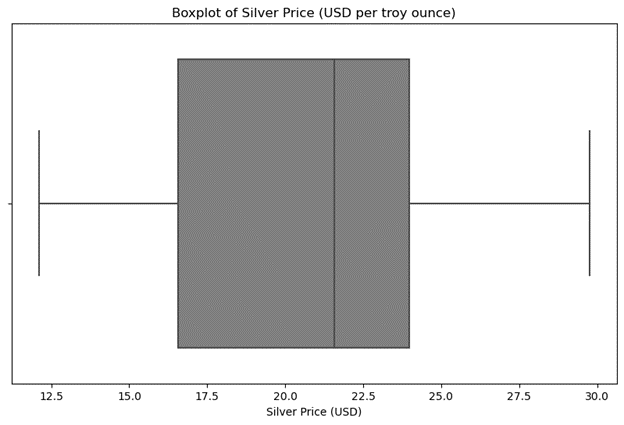
\includegraphics[width=1\textwidth]{bibliography/Figure/boxplot_silver.png}
    \caption{Biểu đồ hộp của giá bạc}
    \label{fig:3}
    \end{minipage}
    \hfill
    \begin{minipage}{0.23\textwidth}
    \centering
    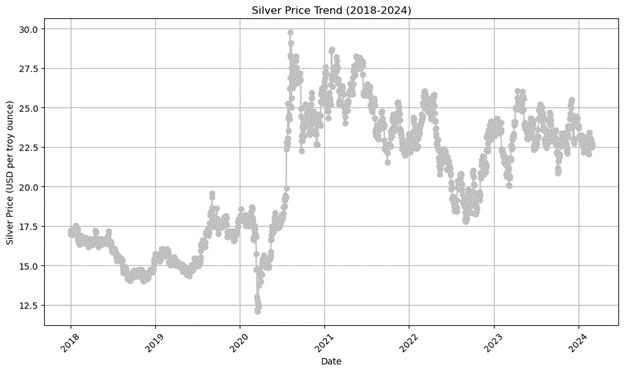
\includegraphics[width=1\textwidth]{bibliography/Figure/line_silver.png}
    \caption{Biểu đồ đường của giá bạc}
    \label{fig:4}
    \end{minipage}
\end{figure} 

\begin{figure}[H]
    \centering
    \begin{minipage}{0.23\textwidth}
    \centering
    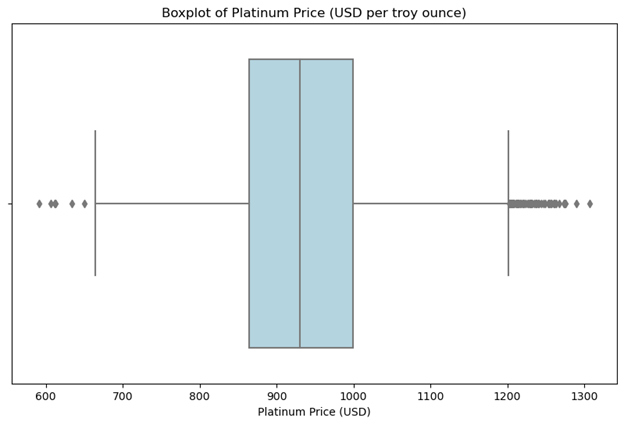
\includegraphics[width=1\textwidth]{bibliography/Figure/boxplot_pt.png}
    \caption{Biểu đồ hộp của giá bạch kim}
    \label{fig:5}
    \end{minipage}
    \hfill
    \begin{minipage}{0.23\textwidth}
    \centering
    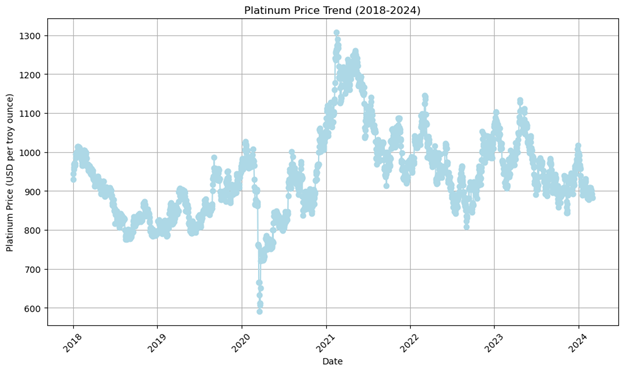
\includegraphics[width=1\textwidth]{bibliography/Figure/line_pt.png}
    \caption{Biểu đồ đường của giá bạch kim}
    \label{fig:6}
    \end{minipage}
\end{figure}




\subsection{Công cụ sử dụng}
Trong quá trình nghiên cứu và phân tích dữ liệu để dự báo giá khoáng sản, nhóm đã sử dụng một số công cụ và thư viện phần mềm phổ biến, chủ yếu được triển khai bằng ngôn ngữ lập trình Python. Danh sách các công cụ và thư viện chính được sử dụng: Pandas, NumPy, Matplotlib, Seaborn, Scikit-learn,... 
\section{Phương pháp} 

\subsection{Linear Regression}
Hồi quy tuyến tính (Linear Regression) được giới thiệu lần đầu bởi nhà thống kê Sir Francis Galton vào cuối thế kỷ 19, là một phương pháp thống kê dùng để mô hình hóa mối liên hệ giữa một biến phụ thuộc và một (hoặc nhiều) biến độc lập. Hồi quy tuyến tính đơn thì có 1 biến độc lập, hồi quy tuyến tính bội thì có nhiều hơn 1 biến độc lập.\\
Nó xây dựng một mô hình tuyến tính bằng cách tìm một đường thẳng (nếu là hồi quy đơn biến) hoặc một siêu phẳng (nếu là hồi quy đa biến) dự đoán tốt nhất dựa trên quan hệ tuyến tính sao cho khác biệt giữa giá trị dự đoán và giá trị thực tế là nhỏ nhất.\\
Hồi quy tuyến tính được ứng dụng rộng rãi để dự đoán giá trị đầu ra, xem xét ảnh hưởng của các biến số trong các lĩnh vực như kinh tế, tài chính, môi trường,...\\
Phương trình hồi quy tuyến tính đơn biến: 
\begin{samepage}
\[Y=\beta_0+\beta_1X_1+\varepsilon\]
\end{samepage}
Phương trình hồi quy tuyến tính bội với k biến độc lập:
\begin{samepage}
\[Y=\beta_0+\beta_1X_1+...+\beta_kX_k+\varepsilon\]
\end{samepage}
Trong đó:\\
        \indent\textbullet\ Y là giá trị dự đoán của biến phụ thuộc (Y) ứng với giá trị các biến độc lập \(X_1, X_2, \ldots, X_k\)\\
        \indent\textbullet\ \(\beta_0\) là hệ số chặn, là giá trị dự đoán của Y khi giá trị của các biến độc lập bằng 0\\
        \indent\textbullet\ \(\beta_1,..., \beta_k\) là hệ số tương quan hồi quy – cho thấy mức độ mạnh yếu trong mối liên hệ của Y với các biến độc lập.\\
        \indent\textbullet\ \(X_1, X_2, \ldots, X_k\) là giá trị các biến độc lập để dự đoán Y.\\
        \indent\textbullet\ \(\varepsilon\) là sai số của dự đoán, là phần biến thiên không thể giải thích bởi mối liên hệ tuyến tính của X và Y.

\subsection{GRU}
Mạng Neural hồi tiếp nút có cổng (GRU) là một cơ chế cổng trong các mạng nơ ron hồi quy, là một biến thể đơn giản hơn của mạng Bộ nhớ ngắn hạn dài (LSTM). GRU có thể xử lý dữ liệu tuần tự như văn bản, bài viết và chuỗi thời gian.
GRU sử dụng cơ chế cổng để cập nhật có chọn lọc trạng thái ẩn của mạng tại mỗi bước thời gian. Cơ chế cổng được dùng để kiểm soát luồng dữ liệu đi vào và đi ra của mạng. GRU có 2 cơ chế cổng: cổng xóa và cổng cập nhật. \\
Cổng xóa quyết định bao nhiêu phần mà trạng thái trước đây được giữ lại, còn cổng cập nhật quyết định trạng thái ẩn mới có bao nhiêu phần giống trạng thái ẩn cũ. Đầu ra của GRU là tính toán dựa trên số trạng thái ẩn được cập nhật, giúp mô hình có thể ‘nhớ’ thông tin quan trọng từ quá khứ và ‘nhìn’ vào thông tin mới để điều chỉnh trạng thái hiện tại.\\ toán cổng xóa, cổng cập nhật, và số trạng thái ẩn của GRU như sau:\\
Cổng xóa:
\[
R_t = \sigma(X_t W_{xr} + H_{t-1} W_{hr} + b_r)
\]
Cổng cập nhật:
\[
Z_t = \sigma(X_t W_{xz} + H_{t-1} W_{hz} + b_z)
\]
Trong đó:\\
\begin{itemize}
    \item $X_t$: đầu vào ở bước thời gian hiện tại.
    \item $H_{t-1}$: là trạng thái ẩn ở bước trước đó.
    \item $W_{xr}, W_{xz} \in \mathbb{R}^{d \times h}$ và $W_{hr}, W_{hz} \in \mathbb{R}^{h \times h}$: là các trọng số.
    \item $b_r, b_z \in \mathbb{R}^{1 \times h}$: là các tham số độ chênh.
    \item $\sigma$: là hàm sigmoid để 2 giá trị thu được thuộc khoảng $(0,1)$.
\end{itemize} 

\vspace{-1em} % Điều chỉnh giá trị này để giảm khoảng cách
\begin{figure}[H]
    \centering
    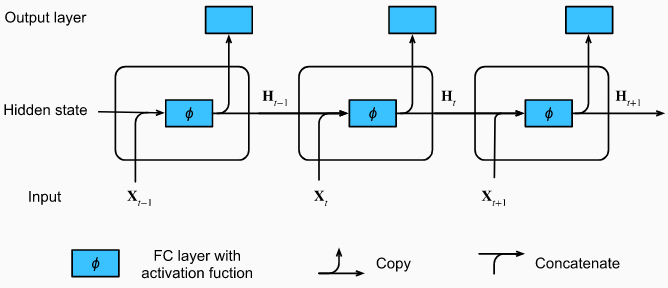
\includegraphics[width=0.5\textwidth]{bibliography/Figure/GRUModel.png}
    \caption{Mô hình GRU}
    \label{fig:GRU_Model}
\end{figure} 

\subsection{PatchTST}
PatchTST là mô hình sử dụng Transformer để dự đoán đa biến và học biểu diễn tự giám sát. Dựa trên hai phần chính: \\
\begin{enumerate}
    \item \textbf{Vá dữ liệu (Patching) :} phân đoạn chuỗi thời gian thành các đoạn nhỏ cấp độ chuỗi con, được sử dụng làm các token đầu vào cho Transformer.
    \item \textbf{Kênh truyền độc lập:} mỗi kênh chứa một chuỗi thời gian đơn biến duy nhất, sử dụng cùng trọng số Transformer và trọng số nhúng trên tất cả các chuỗi. 
\end{enumerate}
Kiến trúc mô hình PatchTST sử dụng bộ mã hóa Transformer gốc, mỗi chuỗi đơn biến có độ dài \( L \) được chia thành các mảnh, đưa vào Transformer một cách độc lập, và tạo ra \( T \) giá trị tương lai \( (x_{L+1}, \ldots, x_{L+T}) \).
\begin{figure}[H]
    \centering
    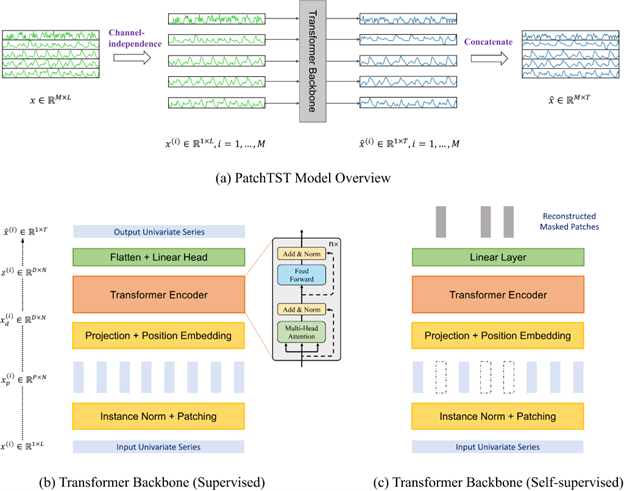
\includegraphics[width=0.5\textwidth]{bibliography/Figure/PatchTSTWorkflow.png}
    \caption{Mô hình PatchTST}
    \label{fig:PatchTST_Model}
\end{figure}
Dữ liệu chuỗi thời gian đa biến \( x \in \mathbb{R}^{M \times L} \) được chia thành các chuỗi đơn biến \( x^{(i)} \in \mathbb{R}^{1 \times L} \) với \( i = 1, \ldots, M \), sau đó được đưa vào Transformer Backbone để xử lý. Các quy trình tiến tới (forward process) là độc lập, và các dự đoán đầu ra \( \hat{x}^{(i)} \in \mathbb{R}^{1 \times T}, i = 1, \ldots, M \) được gộp lại để tạo ra đầu ra cuối cùng \( \hat{x} \in \mathbb{R}^{M \times T} \). 

PatchTST có hai biến thể:
\begin{itemize}
    \item \textbf{PatchTST có giám sát:} Sử dụng dữ liệu có nhãn.
    \item \textbf{PatchTST tự giám sát:} Không yêu cầu dữ liệu có nhãn.
\end{itemize}

\subsection{TBATS}
TBATS là một mô hình dự báo chuỗi thời gian nâng cao, cải tiến từ mô hình BATS, và được phát triển bởi Rob J. Hyndman và Nikolaos Kourentzes. Mô hình TBATS được tạo ra vào năm 2011 với mục đích để dự báo chuỗi thời gian với nhiều chu kỳ mùa vụ (chu kỳ theo giờ, ngày, quý, năm,..). TBATS có thể xử lý các dạng mùa vụ phức tạp như tính mùa vụ không phải số nguyên, không lồng nhau và mùa vụ có chu kỳ dài.
 \\
TBATS thì ít phổ biến và ít được dùng hơn so với các mô hình khác trong phả hệ mô hình ARIMA. TBATS gồm 5 thành phần:\\
\indent\textbullet\ \textbf{Trigonometric seasonality} (tính mùa vụ theo lượng giác): dùng phép biến đổi lượng giác (sin-cos) để mô hình các yếu tố mùa vụ có tần suất cố định.
\\
\indent\textbullet\ \textbf{Box-Cox transformation} (hàm biến đổi Box-Cox): xử lý tính không đồng nhất của dữ liệu, giúp cải thiện phân phối dữ liệu và làm cho phương sai của chúng đồng đều hơn.
\\
\indent\textbullet\ \textbf{ARMA errors} (sai số tự hồi quy kết hợp trung bình trượt): giúp dự đoán các sai số ngẫu nhiên không có tính mùa vụ.\\
\indent\textbullet\ \textbf{Trend components} (xu hướng): thể hiện mô hình dự đoán xu hướng tăng, giảm.\\
\indent\textbullet\ \textbf{Seasonal components} (các yếu tố mùa vụ): loại bỏ các biến động chu kỳ khỏi dữ liệu.
\\
Công thức:\\
\begin{itemize}
    \item \textbf{Hàm biến đổi Box-Cox:}
    \begin{itemize}
        \item Trường hợp tuyến tính:
        \[
        y_t^{(\omega)} =
        \begin{cases}
        \frac{y_t^\omega - 1}{\omega}, & \omega \neq 0 \\
        \log y_t, & \omega = 0
        \end{cases}
        \]
        \[
    y_t^{(\omega)} = l_{t-1} + \phi b_{t-1} + \sum_{i=1}^{T} s_{t-m_i}^{(i)} + d_t
    \]

        \item Trường hợp phi tuyến tính:
        \[
        y_t^{(\omega)} = w' x_{t-1} + \varepsilon_t
        \]
        \[
        x_t = F x_{t-1} + g \varepsilon_t
        \]

        Trong đó, \( m_1, \ldots, m_T \) nói về chu kỳ mùa, \( l_t \) là mức riêng của chu kỳ \( t \), \( st^(i) \) biểu diễn cho thành phần mùa vụ tại thời điểm \( t \), \( \mathbf{w'} \) là một dòng véc-tơ, \( \mathbf{g} \) là một cột véc-tơ, \( \mathbf{F} \) là một ma trận và \( \mathbf{x}_t \) là véc-tơ trạng thái không quan sát được tại thời điểm\( t \) (tương lai). 
    \end{itemize}
    \item \textbf{Hàm xử lý với phương pháp làm mịn – giảm đà xu hướng (trend damping), tìm các hệ số ARMA, mức riêng.}
    \begin{align*}
    l_t &= l_{t-1} + \phi b_{t-1} + \alpha d_t \\
    d_t &= \sum_{i=1}^{p} \varphi_i d_{t-i} + \sum_{i=1}^{q} \theta_i \varepsilon_{t-i} + \varepsilon_t \\
    b_t &= (1 - \phi)b + \phi b_{t-1} + \beta d_t
    \end{align*}
    Trong đó, \( b_t \) là xu hướng ngắn hạn trong chu kỳ \( t \), \( d_t \) nói về hệ số ARMA(\( p \), \( q \)) và sai số \( \varepsilon_t \) lấy từ quá trình nhiễu trắng với trung bình bằng 0 và phương sai cố định \( \sigma^2 \), \( \alpha \) và \( \beta \) và \( \gamma_i \) (\( i = 1, \ldots, T \)) là các hệ số làm mịn, \( \theta_i \) là hệ số thành phần i của trung bình trượt (MA). Xu hướng làm mịn Gardener & McKenzie với tham số \( \phi \) được sử dụng theo hướng Snyder để tạo nên \( b_t \).


    \item \textbf{Hàm biến đổi lượng giác:}
    \[
    s_t^{(i)} = \sum_{j=i}^{k_i} s_{j,t}^{(i)}
    \]
    \[
    k_i = 
    \begin{cases} 
    \frac{m_i}{2} & \text{nếu giá trị của mùa i là chẵn,} \\
    \frac{(m_i - 1)}{2} & \text{nếu giá trị của mùa i là lẻ}
    \end{cases}
    \]
    \begin{align*}
    s_{j,t}^{(i)} &= s_{j,t-1}^{(i)} \cos \lambda_j^{(i)} + s_{j,t-1}^{*(i)} \sin \lambda_j^{(i)} + \gamma_1^{(i)} d_t \\
    s_{j,t}^{*(i)} &= -s_{j,t-1} \sin \lambda_j^{(i)} + s_{j,t-1}^{*(i)} \cos \lambda_j^{(i)} + \gamma_2^{(i)} d_t \\
    \lambda_j^{(i)} &= 2\pi j / m_i
    \end{align*}
Trong đó, \( \gamma_1 \) và \( \gamma_2 \) là tham số làm mịn, \( s_{j,t}^{(i)} \) là mức độ tăng trưởng ngẫu nhiên trong khoảng thời gian \( s_j^{*(i)} \).


\end{itemize}





\begin{figure}[H]
    \centering
    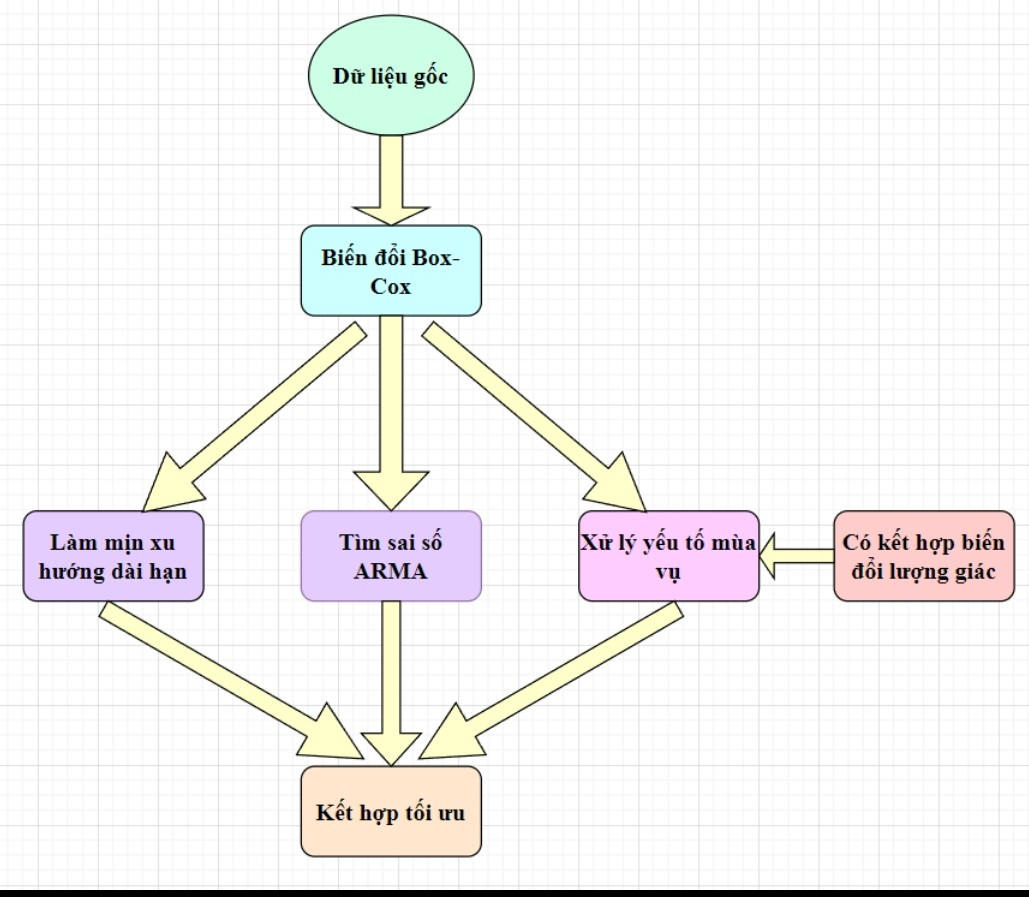
\includegraphics[width=0.5\textwidth]{bibliography/Figure/tbats.png}
    \caption{Hình luồng hoạt động của mô hình TBATS}
    \label{fig:tbats_workflow}
\end{figure}

\textbf{Lưu ý}: để có được mô hình TBATS cuối cùng thì có thể thêm hoặc bỏ các phần xử lý: biến đổi Box-Cox, làm mịn xu hướng (Trend Damping), tính sai số ARMA nhằm tạo được mô hình tốt nhất.

\section{Kết quả thực nghiệm}
\subsection{Các phương pháp đánh giá}
\begin{enumerate}
    \item \textbf{Mean Absolute Percentage Error} (MAPE) là trung bình cộng phần trăm độ lệch tuyệt đối giữa giá trị dự đoán và giá trị thực.
    \begin{align*}
    MAPE &= \frac{1}{n} \sum_{i=1}^n \left|\frac{y_i - \hat{y}i}{y_i}\right| \cdot 100 \
    \end{align*}
    \item \textbf{Root Mean Square Error} (RMSE) là căn bậc hai của trung bình bình phương độ lệch giữa giá trị dự đoán và giá trị thực tế.
    \begin{align*}
    RMSE &= \sqrt{\frac{1}{n} \sum_{i=1}^n (y_i - \hat{y}i)^2} \
    \end{align*}
    \item \textbf{Mean Average Error} (MAE) là trung bình độ lệch tuyệt đối giữa giá trị dự đoán và giá trị thực tế.
    \begin{align*}
    MAE &= \frac{1}{n} \sum_{i=1}^n |y_i - \hat{y}i| \
    \end{align*}
\end{enumerate}

\indent Trong đó:
\begin{itemize}
    \item $n$ là tổng số quan sát
    \item $y_i$ là giá trị thực tế của quan sát thứ i.
    \item $\hat{y}_i$ là giá trị dự đoán của quan sát thứ i.
\end{itemize}


\subsection{Kết quả thực nghiệm và đánh giá}

\section{Kết luận}

\indent Xét theo chiều ngang, với dữ liệu giá vàng thì tỉ lệ tốt nhất cho các mô hình là 7:3 với số lần có kết quả tốt nhất là 5, tỉ lệ tốt thứ hai là 8:2 (4 lần), kém nhất là tỉ lệ 9:1 (1 lần). Tương tự với dữ liệu giá bạch kim thì tốt nhất là tỉ lệ 8:2 (5 lần), tiếp đó là tỉ lệ 9:1 (4 lần) và 7:3 (1 lần). Với dữ liệu giá bạc thì kém nhất là tỉ lệ 7:3 (2 lần) và 9:1 (3 lần) và tốt nhất là tỉ lệ 8:2 (5 lần). Như vậy tỉ lệ tốt nhất cho toàn bộ dữ liệu là 8:2.

\indent Xét theo chiều dọc, trong với mỗi tỉ lệ, ứng với mỗi phương pháp kiểm định, nhóm nghiên cứu sẽ chọn ra 3 mô hình dự báo tốt nhất; top 1, 2, 3, sẽ được gán hệ số 3, 2, 1 và mô hình nào có tổng hệ số cao nhất thì chọn. Từ đó, chọn ra 3 mô hình tốt nhất của mỗi bộ dữ liệu.

\begin{table}[h!]
    \centering
    \resizebox{0.48\textwidth}{!}{
    \renewcommand{\arraystretch}{1.5}
    \small
    \begin{tabular}{|c|c|c|c|c|c|}
        \hline
        \textbf{Bộ dữ liệu} & \textbf{Xếp hạng} & \textbf{Tỉ lệ 7:3} & \textbf{Tỉ lệ 8:2} & \textbf{Tỉ lệ 9:1} & \textbf{3 mô hình tốt nhất} \\ \hline
        \multirow{3}{*}{Giá vàng} & Top 1 & GRU (9) & GRU (9) & LSTM (9) & GRU \\ \cline{2-6} 
                                  & Top 2 & RNN (6) & RNN (6) & GRU (6) & RNN \\ \cline{2-6} 
                                  & Top 3 & LSTM (3) & LSTM (3) & RNN (3) & LSTM (top 2) \\ \hline
        \multirow{3}{*}{Giá bạch kim} & Top 1 & LSTM (8) & GRU (9) & GRU (8) & GRU \\ \cline{2-6} 
                                      & Top 2 & GRU (7) & LSTM (6) & LSTM (7) & LSTM \\ \cline{2-6} 
                                      & Top 3 & RNN (3) & RNN (3) & RNN (3) & RNN \\ \hline
        \multirow{3}{*}{Giá bạc} & Top 1 & GRU (9) & GRU (9) & GRU (9) & GRU \\ \cline{2-6} 
                                 & Top 2 & LSTM (6) & RNN (6) & LSTM (6) & LSTM \\ \cline{2-6} 
                                 & Top 3 & RNN (3) & LSTM (3) & RNN (3) & RNN \\ \hline
    \end{tabular}}
    \caption{\centering Bảng xếp hạng các mô hình được đánh giá theo chiều dọc}
    \label{table:models}
\end{table}

\indent Cuối cùng sau khi xét theo chiều dọc, từ những mô hình được chọn là tốt nhất trong cả ba bộ dữ liệu thì nhóm nhận thấy mô hình tốt nhất là GRU. Trong số những mô hình được kỳ vọng sẽ cho ra kết quả tốt thì chỉ có mô hình LSTM được chọn là tốt, còn mô hình ARIMA và TBATS thì có kết quả dự đoán không thực sự tốt. Trong cả 3 mô hình tốt nhất thì luôn là GRU, LSTM, RNN và đều là thuật toán học sâu và kết quả chênh lệch nhau không quá lớn, điều này cho thấy các thuật toán dạng này cho ra kết quả khả quan hơn cho các bộ dữ liệu giá khoáng sản này, PatchTST và N-HiTS cũng cho ra kết quả khá tốt khi kết quả luôn không quá lệch so với top 3.

\indent Như vậy, mô hình GRU theo kết quả thì cho thấy khả năng học tuyệt vời với tiềm năng dự đoán giá ba loại kim loại quý trong tương lai. Từ kết quả này, các nhóm nghiên cứu và nhà phân tích dữ liệu trong tương lai có thể cân nhắc về những mô hình có thể dự đoán tốt và mở rộng nghiên cứu dự đoán cho cả các loại kim loại khác hoặc lĩnh vực khác có liên quan cũng như cải tiến mô hình nhằm phục vụ tốt hơn cho các nhu cầu học thuật và kinh doanh.